\documentclass[runningheads,a4paper]{llncs}
\usepackage{graphicx}
\usepackage{hyperref}
\usepackage{float}

\begin{document}

\title{CS32310: Advanced Computer Graphics Assignment 2016--2017 — Scene Modelling and Navigation}
\titlerunning{CS32310: Assignment 2016--2017}

\author{Owen Garland}

\authorrunning{CS32310: Assignment 2016--2017}

\institute{Department of Computer Science,\\ Llandinam Building, Aberystwyth University,\\ Aberystwyth, Ceredigion, SY23 3DB}

\maketitle
\newpage

\section{Running the Application}
Build instructions can be found in the README.md. Or you can view the project online at \href{http://uni.owen.cymru}{uni.owen.cymru}.

\section{Creating the Application}
  The first thing that I did was to embed my ThreeJS application inside of a website, this allowed me to develop the application in the same way that I am used to working, as well as allowing me to abstract functionality for the application into several javascript files, use ES6 transcompiling to ES5, and it also gave me access to the npm repository to easily download and manage libraries. 

  I used the excellent `canvas-testbed' package to create the HTML page + canvas for my application automatically; I had done it manually, however this was a cleaner solution and provided better CSS\@. I then used the `three' and `three-orbit-controls' packages to import the ThreeJS libraries I needed. 

  My plan was to recreate my bedroom in three dimensions, to start out I placed a series of Points on the canvas that highlighted the X, Y and Z axis. This helped me to visualise the different dimensions and orientate myself to the scene before I had actually built anything that I could use as a reference point. 
  
  \begin{figure}[H]
    \centering
    
\includegraphics[width=0.5\textwidth]{images/1.png}
    \caption{Vertices plotted to show axis}
    \label{fig:window}
  \end{figure}

  The next thing I added was orbit controls, this allows the user to interact with the scene using a mouse and keyboard. This is essential to do whilst developing 3D models, as otherwise you have no easy way of viewing the models you have created quickly. 

  From here I attempted to manually create the walls and floors with Vertices and faces, however this proved to be a very slow method of building objects and I was keen to get something visual to work on top of. 

  This lead me to create my walls and floors with primitive shapes (this can be seen in the objects.js file), this was a lot quicker to develop and allowed me to finally have a room on display. 

  \begin{figure}[H]
    \centering
    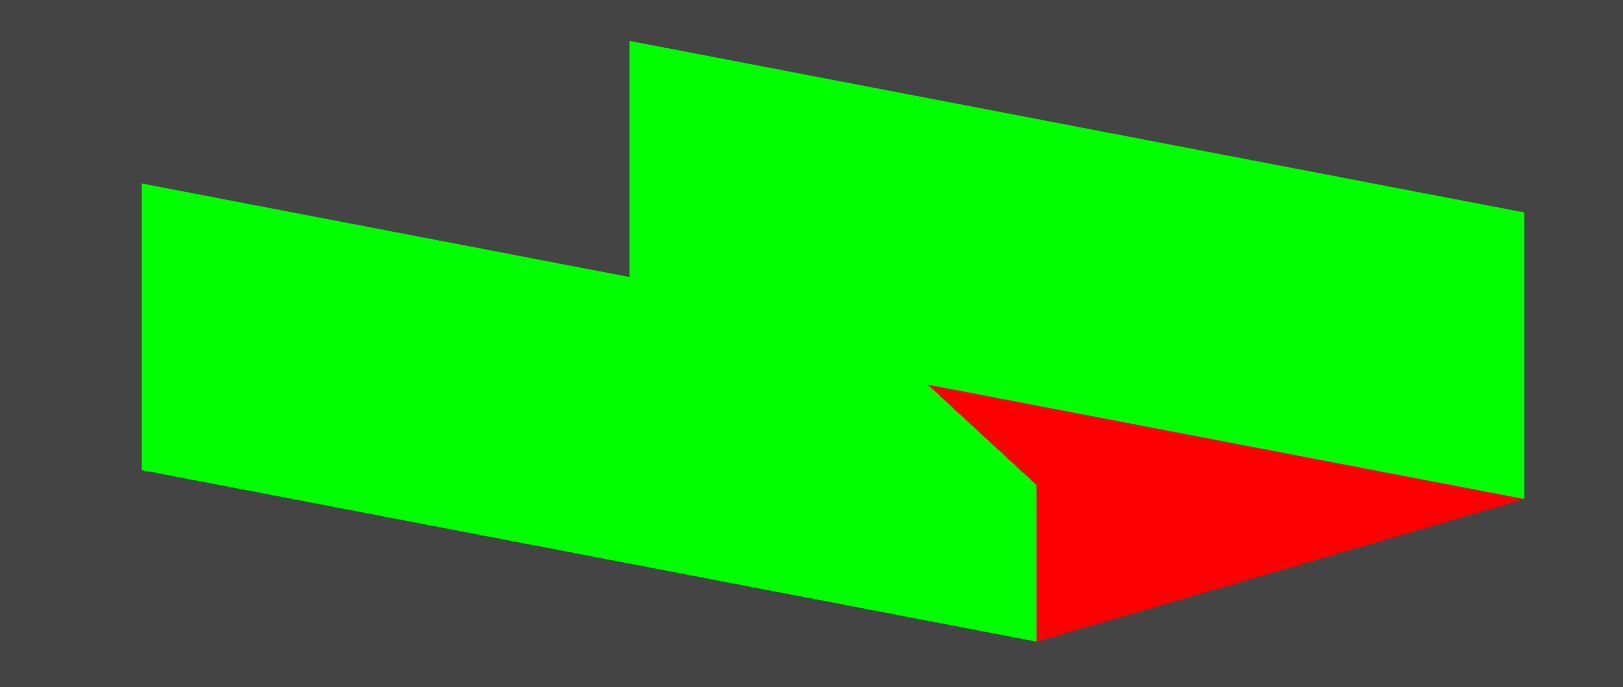
\includegraphics[width=0.5\textwidth]{images/2.png}
    \caption{Basic walls using primitives}
    \label{fig:window}
  \end{figure}
  
  Once I had some walls, and floor I added in texture and lighting effects. I used MeshLambertMaterial and some freely available textures that closely matched my actual bedrooms wall and flooring.

  \begin{figure}[H]
    \centering
    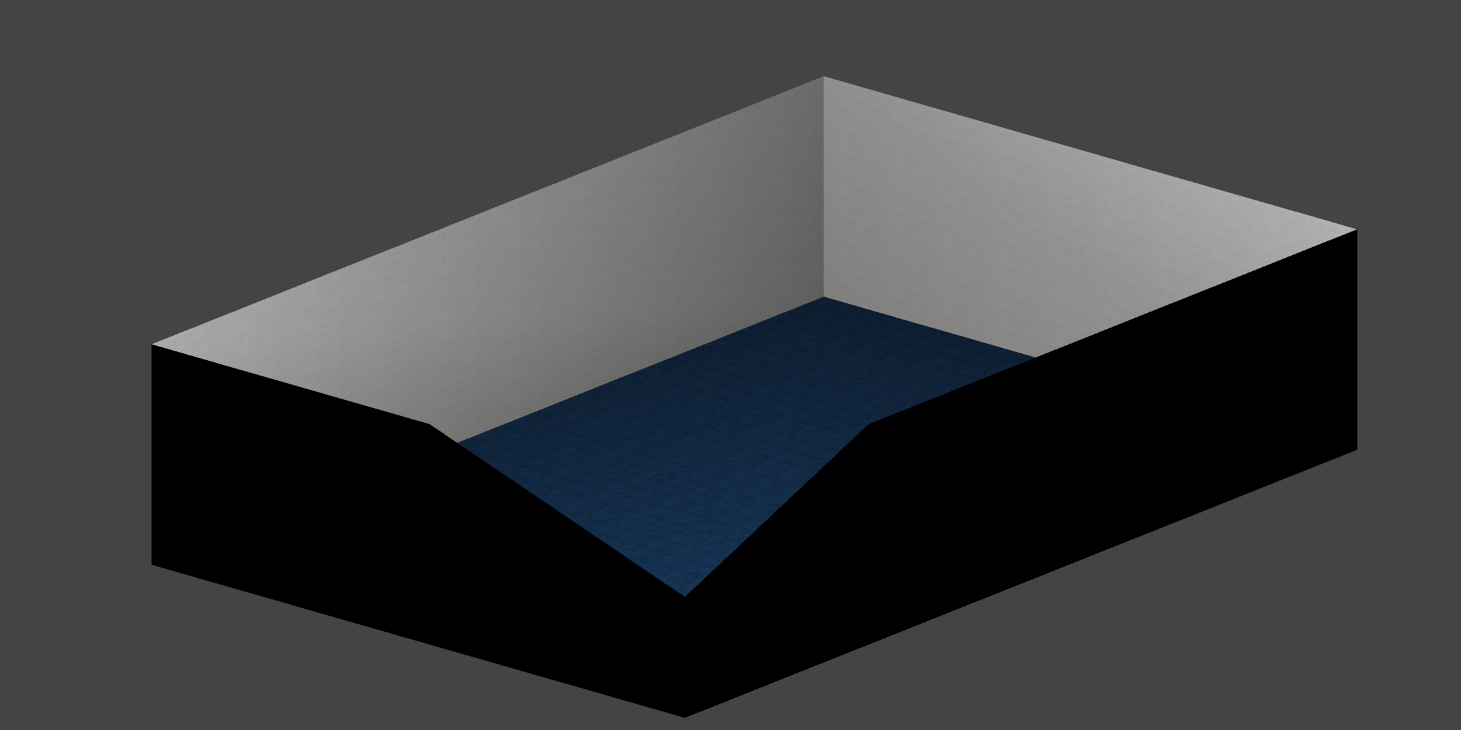
\includegraphics[width=0.5\textwidth]{images/3.png}
    \caption{Walls + floors with textures}
    \label{fig:window}
  \end{figure}

  Once I had a room setup it was time to add some furniture, I decided that it wouldn't be time efficient to manually model these large items myself, so I used the online \href{https://threejs.org/editor/}{three.js editor} to create a bed frame and a door.
  These objects were then exported to JSON, which I was then able to add to my project and load in via the Three.js ObjectLoader function. 

  \begin{figure}[H]
    \centering
    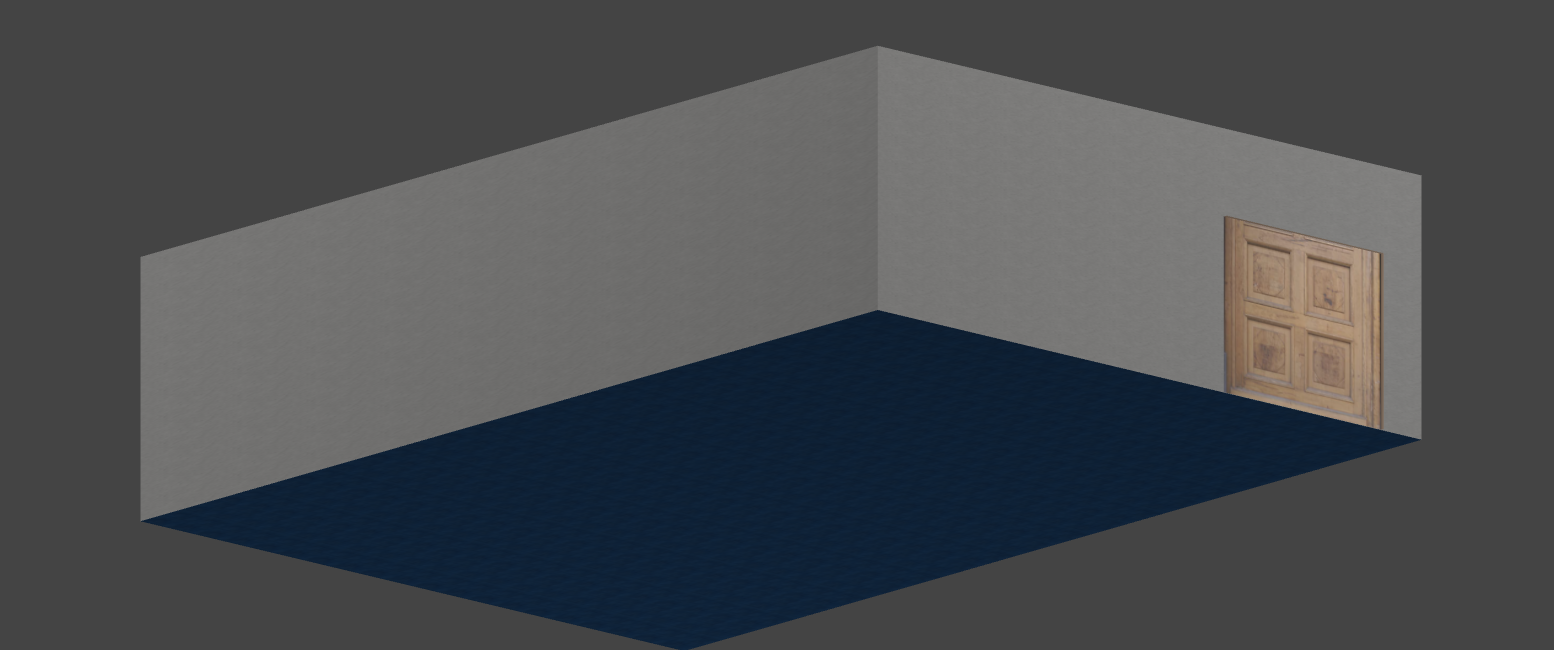
\includegraphics[width=0.5\textwidth]{images/4.png}
    \caption{Scene with imported door object}
    \label{fig:window}
  \end{figure}


  After seeing how easy it was to model objects in the three.js editor I decided to model my whole room this way. Creating the floor, walls, lighting and furniture was a lot easier this way so I quickly replaced the manually developed version (The code is still there though) with one ObjectLoader call that loads in the whole scene from a JSON file. 

  \begin{figure}[H]
    \centering
    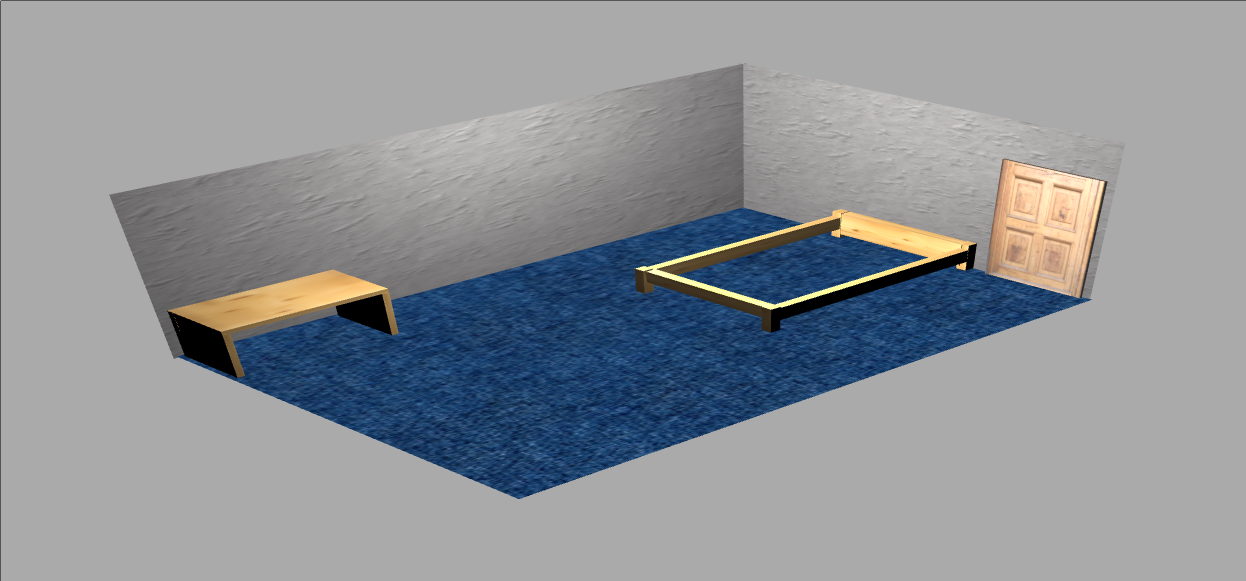
\includegraphics[width=0.5\textwidth]{images/5.png}
    \caption{Imported scene with additional furniture}
    \label{fig:window}
  \end{figure}

  This approach seems a lot simpler and cleaner from an implementation standpoint, although I know that for this assignment you want to see us using primitives and vectors, so I have left the original code in the project which does produce effectively the same output as the code that loads in the scene from the editor. 

  Now that I had multiple objects in my room the lack of shadows was very noticeable, so the next step was to add shadows. I did this by enabling the shadowMap in the renderer and setting objects to receive and cast shadows.

  \begin{figure}[H]
    \centering
    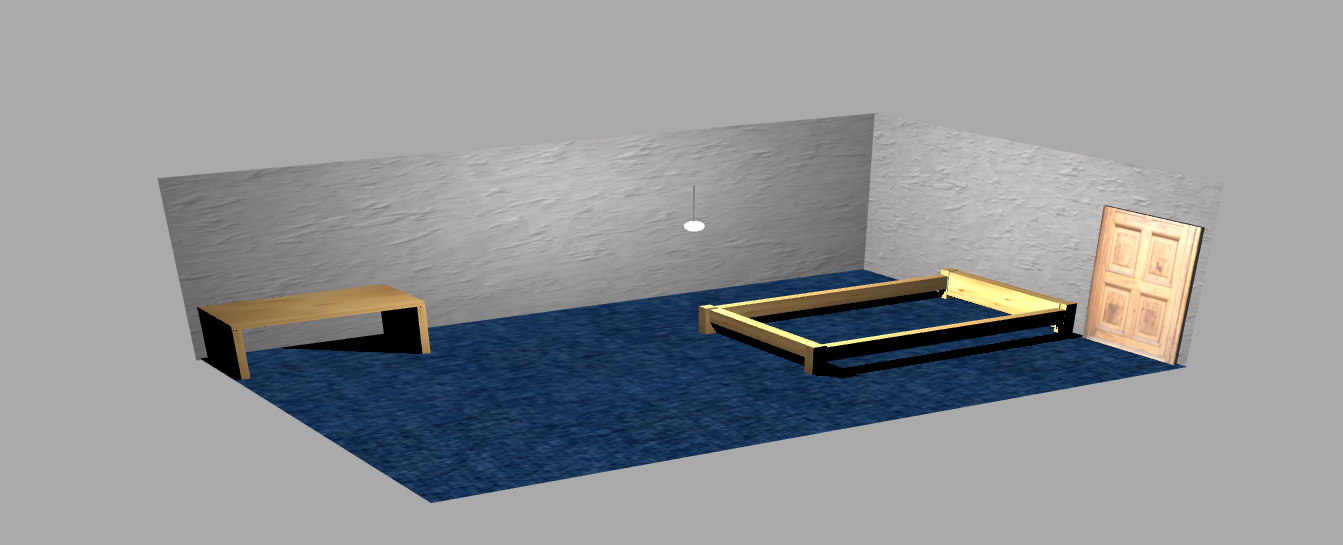
\includegraphics[width=0.5\textwidth]{images/6.png}
    \caption{Added shadows to the scene}
    \label{fig:window}
  \end{figure}

  I then decided to create my own complex shape, I decided upon the coffee mug on my desk. I first created a hollow cylinder to form the walls of the mug, then created a flat cylinder to form the base. To get the different cylinders to match up I shifted the vertices all down by the Y axis to meet with the end of the mug walls. I was then able to merge the geometries to create one whole mug geometry. 

  \begin{figure}[H]
    \centering
    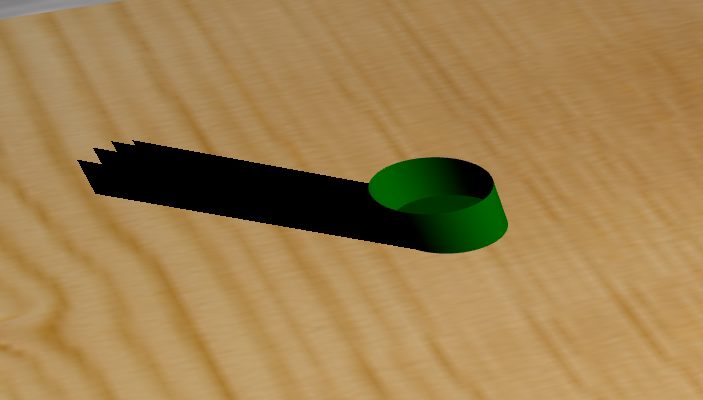
\includegraphics[width=0.5\textwidth]{images/7.png}
    \caption{Coffee mug using two primitives merged together}
    \label{fig:window}
  \end{figure}


  I added a green material texture and set the mug to receive and cast shadows, however when I had both of these options there appeared to be some rendering errors, so I had to opt to turn off the receiving shadows. The shadows on the desk also didn't play well with the desk texture, which lead to very blocky shadows.

  I now wanted to create my own handle for the mug using vertices I plotted myself. This proved to be rather challenging. My plan was to use a sine curve to generate a wave of points, then select one curve of the wave to use as my handle. I was able to this and generate four waves to make each side of the handle.

  \begin{figure}[H]
    \centering
    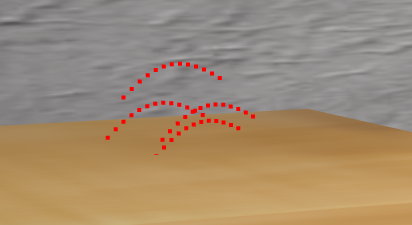
\includegraphics[width=0.5\textwidth]{images/8.png}
    \caption{Vertices plotted to make a handle}
    \label{fig:window}
  \end{figure}

  With the vertices created I now needed to add faces to them to create a wireframe that a material could be applied to. Unfortunately this is where I was unable to find a suitable solution. I could have manually added each face to the geometry but this seemed like an incorrect way of doing things as it would have been repeating code and been a painstaking manual process. 

  Instead I opted to use the triangulateShape function provided from three.js, this did allow me to create faces on the points, however I couldn't manage to get them to be created in the positions that I had imagined. 

  \begin{figure}[H]
    \centering
    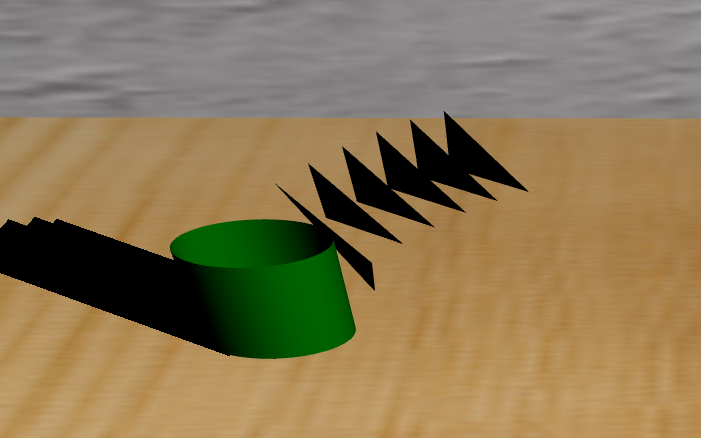
\includegraphics[width=0.5\textwidth]{images/9.png}
    \caption{Faces added to handle, but obviously not how I intended}
    \label{fig:window}
  \end{figure}

  Overall I think this project went fairly well. I wish I had more time to have sorted out the handle, and added in some animations, but I do feel pleased to have learned the basics of how to use three.js to create 3D interactive scenes. I think in reality most people would use a 3D editor like blender to create their objects / scene then export it into JSON and just use three.js to make it interactive and accessible via the web. 

\end{document}
